\documentclass[UTF8]{ctexart}
\usepackage{ctex}
\usepackage{geometry}
\usepackage{enumitem}
\usepackage{indentfirst}
\usepackage{color}
\usepackage{fancyhdr}
\usepackage{amsmath}
\usepackage{graphicx}
\usepackage{amssymb}
\usepackage{tikz}
\usepackage{cases}
\usepackage{array}
\usepackage{pgfplots}
\usepackage{tkz-euclide}
\usepackage{mathrsfs}
% 设置纸张和页边距——A4
\geometry{papersize={21cm,29.7cm}}
\geometry{left=3.18cm,right=3.18cm,top=2.54cm,bottom=2.54cm}

% 一级标题靠左
\CTEXsetup[format={\Large\bfseries}]{section}

% 去除页眉
\pagestyle{plain}

%设置段间距
\addtolength{\parskip}{.4em}
%%设置行间距
%\usepackage{setspace}
%\setstretch{2.5}

% 开始文档内容
\begin{document}

\title{信号与系统课程笔记:Lecture 17 \\
香农-奈奎斯特(Shannon–Nyquist)采样定理}
\author{授课教师:秦雨潇 \\
        笔记记录:曹时成}
\date{2023 年 11 月 10 日(第十周,周五)}
\maketitle

\section{课堂回顾}

\subsection{零输入响应和零状态响应}
傅里叶变换只能求零状态响应 \par
\subsection{无失真传输与理想低通滤波器}
\begin{figure}[h]
    \centering         %使图片居中放置
    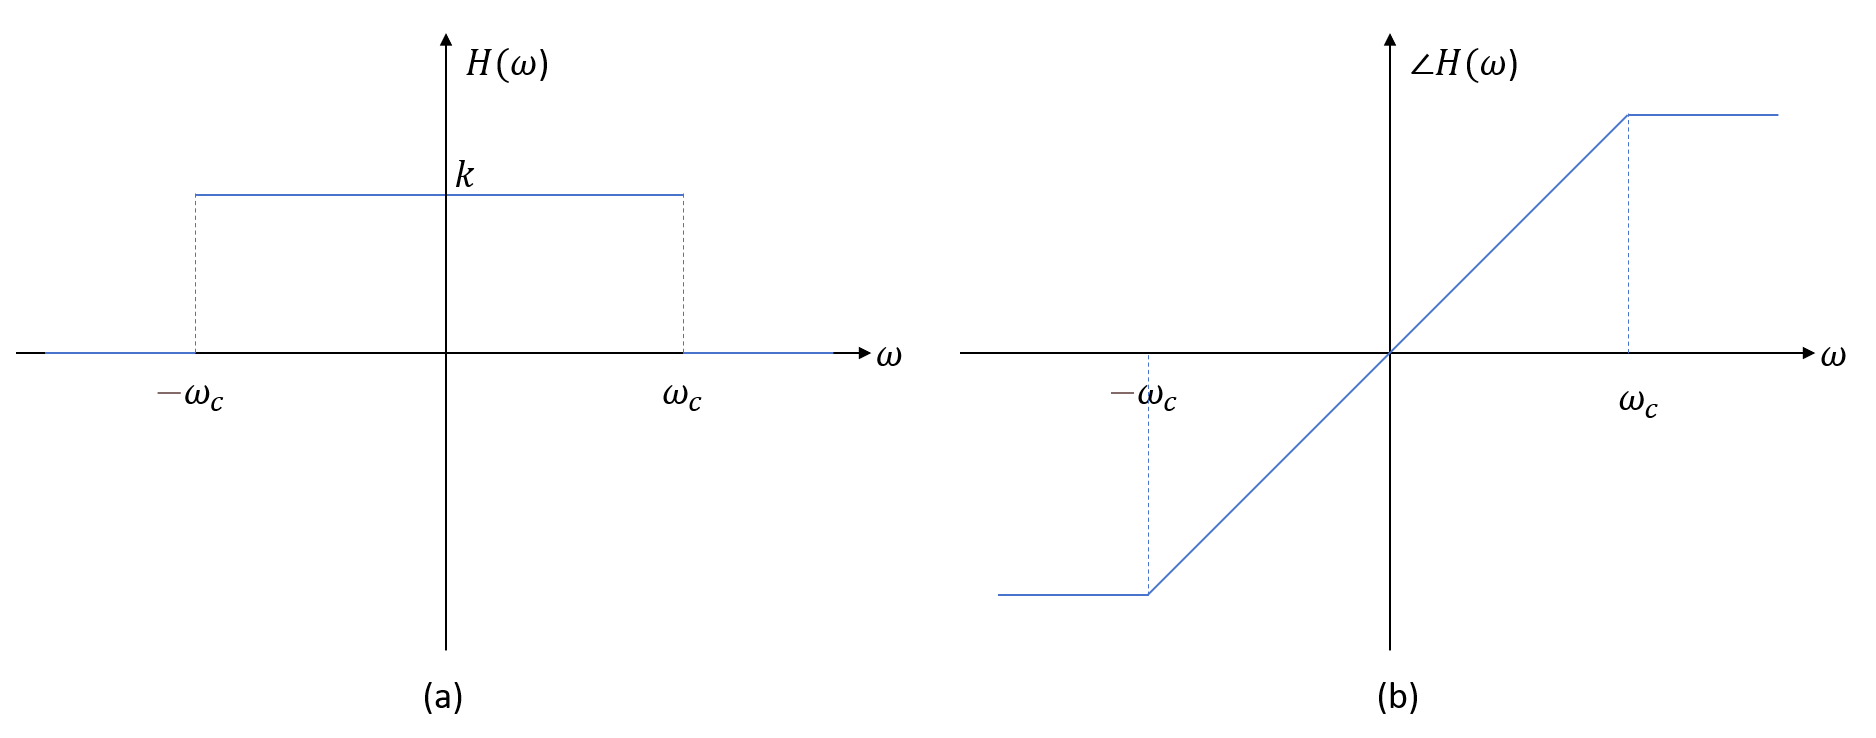
\includegraphics[scale=0.32]{1.png}
    \caption{理想低通滤波器在频域的表示。(a)幅频;(b)相频。}
\end{figure}
在“有限带宽”$[-w_c,w_c] $范围内,满足: \par
\[  H(w) =\left\{ \begin{array}{rcl}
    ke^{-jwt_d}, & & {w\leqslant w_c}\\
    0, & & {{w> w_c}}\\
    \end{array} \right. \] \par
$t_d$ 为时间延迟 \par
$ \mathscr{F}^{-1}\{ H(w)\} =\frac{w_c}{\pi}Sa[w_c (t-t_d)]  $ \par
表明:理想低通滤波器在频域上是门函数,在时域上是 Sa 函数,且在时域上 Sa 函数关于 $t_d$ 对称。
\subsection{如何理解 Ideal LPF 的“物理不可实现性”?}
(1)$ \mathscr{F}^{-1}{H(w)}$ 是Sa函数,在时间上趋向于无穷时,仍然有信号,这是不存在的。\par
(2)$\delta _t\rightarrow h(t)$,表明 Sa 函数在$t<0$时也有信号,这是“非因果”的。 \par
\subsection{ Ideal LPF 的其他性质}
$\delta _t\rightarrow A\delta (t-t_d)$,信号是从$\delta$函数变为 Sa 函数,信号不是一个无失真系统,信号是“严重失真”的。\par
\subsection{物理可实现的理想低通滤波器的条件}
“佩利-维纳”定理 \qquad  是一个“必要条件”\par
(1)在时域上:$h(t)=0$ \quad for \quad  $t<0$\par
(2)在频域上:\par
A.\quad $\int_{\mathbb{R}}| H(w)\vert^2dw<\infty\equiv \int_{\mathbb{R}}| h(t)\vert^2dw<\infty\ $\par
B.\quad $\int_{\mathbb{R}}\frac{ln| H(w)\vert }{1+w^2} dw<\infty\ $,表明衰减不能快于$e^{-w^2}$\par
\section{采样定理}
见对应的课件“信号与系统-采样定理”\par
\section{例2}
$y''(t)+5y'(t)+6y(t)=2f'(t)+6f(t)$,其中,$y(0_-)=1$,$y'(0_-)=-1$,$f(t)=5costu(t)$\par
解:进行拉普拉斯变换可得:\par
\qquad $Y(s)=\frac{s^2y(0_-)+y'(0_-)+sy(0_-)}{s^2+5s+6} +\frac{2(s+3)}{s^2+5s+6}F(s) $\par
对于这个完全响应:\par
\qquad 第一项$\frac{s^2y(0_-)+y'(0_-)+sy(0_-)}{s^2+5s+6}$为“零输入响应”项\par
\qquad 第二项$\frac{2(s+3)}{s^2+5s+6}F(s)$为“零状态响应”项\par
\qquad 分母$s^2+5s+6$为“系统”\par
\qquad 第一项分子$s^2y(0_-)+y'(0_-)+sy(0_-)$为“初始条件”\par
\qquad 第二项分子$2(s+3)F(s)$为“激励”\par
对$Y(s)$化简得:$Y(s)=\frac{k_1}{s+2}+\frac{k_2}{s+3}+\frac{k_3}{s+2}+\frac{k_4}{s+1} $\par
\qquad $\mathscr{L}^{-1}{Y(s)}=[ k_1e^{-2t}+k_2e^{-3t}+k_3e^{-2t}+k_4cos(t-\varphi _4)]u(t) $\par
其中前两项为“零输入”响应,后两项为“零状态”响应;前三项也称为“暂态分量”,最后一项也称为“稳态分量”。
\end{document}